\documentclass[12pt,a4paper]{ctexart}

\usepackage[a4paper,margin=2.5cm]{geometry}
\usepackage{setspace}
\usepackage{array}
\usepackage{longtable}
\usepackage{graphicx}
\usepackage{fancyhdr}
\usepackage{titling}
\usepackage{enumitem}
\usepackage{amsmath,amssymb}
\usepackage{bm}
\usepackage{booktabs}
\usepackage{caption}
\usepackage{float}
\usepackage{hyperref}
\usepackage{listings}
\usepackage[dvipsnames, svgnames, x11names]{xcolor}

\lstset{
	backgroundcolor=\color[rgb]{0.96,0.96,0.96},
	keywordstyle=\color{blue}\bfseries,
	identifierstyle=\color{black},
	commentstyle=\color[rgb]{0,0.6,0},
	stringstyle=\color[rgb]{0.58,0,0.82},
	basicstyle=\small\ttfamily,
	columns=fullflexible,
	breaklines=true,
	captionpos=t,
	tabsize=4,
	morekeywords={},
	emph={self},
	emphstyle=\bfseries\color{Rhodamine},
	frame=lines,
	framesep=1em,
	rulesepcolor=\color{red!20!green!20!blue!20},
	language=Python,
	numbers=left,
	showstringspaces=false,
	numberstyle=\footnotesize,
	extendedchars=false,
	xleftmargin=3em
}

\setlength{\parindent}{2em}
\setlength{\parskip}{0.5em}
\renewcommand{\arraystretch}{1.5}
\linespread{1.3}

\pagestyle{fancy}
\fancyhf{}
\cfoot{\thepage}
\renewcommand{\headrulewidth}{0pt}

% ===== 可修改信息 =====
\newcommand{\schoolname}{数学与统计学院}
\newcommand{\classname}{数学强基2301}
\newcommand{\studentid}{2233210080}
\newcommand{\studentname}{袁浩然}
\newcommand{\teachername}{孟德宇老师}
\newcommand{\labplace}{数学实验中心}
\newcommand{\experimenttitle}{SVM 算法解决二/多分类问题}
\newcommand{\schoolyear}{2023--2024学年\quad 第二学期}
\usepackage{fancyhdr}

% 设置 fancyhdr 样式
\fancypagestyle{plain}{
	\fancyhf{} % 清除所有预设的页眉和页脚
	\renewcommand{\headrulewidth}{0pt} % 如果不需要页眉线
	\renewcommand{\footrulewidth}{0pt} % 如果不需要页脚线
}

% 应用新的 plain 样式到所有页面
\pagestyle{plain}

\begin{document}
	
	\section*{实验二：SVM 算法解决二/多分类问题}
	
	\section*{一、实验内容}
	这次实验我做的是支持向量机在多分类任务上的实现。根据要求，本实验分别实现了二分类 SVM、One-vs-Rest 和 One-vs-One 两种多分类策略，然后在人工生成的三分类数据集上做训练和测试。
	
	整个实验主要包括这几个部分：先生成带有三个类别的二维数据；然后把数据划分为训练集和测试集，并做标准化处理；接着训练多分类 SVM 模型；最后用准确率、混淆矩阵和分类边界图来观察模型效果。因为这次实验强调可视化，所以我把数据分布、决策区域和混淆矩阵都画了出来，结果看起来也比较直观。
	
	\section*{二、问题描述与原理}
	支持向量机本质上是通过寻找一个最优超平面来完成分类任务。对于线性可分或近似线性可分的数据，它希望在分类正确的同时，让两类样本到分割面的间隔尽可能大。这样做的好处是模型一般会有更好的泛化能力。
	
	对于二分类问题，线性 SVM 的判别函数可以写成：
	\[
	f(x)=w^Tx+b
	\]
	其中 $w$ 是法向量，$b$ 是偏置项。分类时只需要看 $f(x)$ 的符号即可。当标签记为 $y\in\{-1,+1\}$ 时，常见的 hinge loss 形式可以写成：
	\[
	L = \frac{\lambda}{2}\|w\|^2 + \sum_{i=1}^{n}\max\bigl(0,1-y_i(w^Tx_i+b)\bigr)
	\]
	前一项控制模型复杂度，后一项约束分类间隔。训练时，本实验采用了逐样本更新的方式来近似做梯度下降。
	
	因为实验是三分类任务，所以本实验又在二分类 SVM 的基础上扩展了多分类策略：
	\begin{itemize}
		\item[(1)] \textbf{One-vs-Rest（OvR）}：每个类别分别和其余类别做一次二分类，一共训练 $K$ 个分类器，预测时选择得分最大的类别；
		\item[(2)] \textbf{One-vs-One（OvO）}：任意两类之间训练一个二分类器，一共训练 $K(K-1)/2$ 个分类器，预测时通过投票决定最终类别。
	\end{itemize}
	
	我这次主要展示的是 OvO 的结果。因为三分类时只需要训练 3 个二分类器，逻辑比较清楚，而且从图上也能比较明显地看出每块区域是怎么分开的。
	
	关于 SVM 的具体介绍以及学习笔记，我已经将其放在文件夹中。
	
	\section*{三、实验步骤}
	\begin{enumerate}
		\item 人工生成三类二维样本，每一类都围绕一个中心点随机分布；
		\item 将数据按 7:3 划分为训练集和测试集；
		\item 对训练集和测试集做标准化，避免不同维度量纲影响分类结果；
		\item 编写线性二分类 SVM，包括参数初始化、决策函数和预测函数；
		\item 在二分类模型基础上实现 OvR 和 OvO 两种多分类策略；
		\item 设定学习率、正则化系数和训练轮数，对模型进行训练；
		\item 在测试集上计算准确率和 Macro-F1，并绘制混淆矩阵；
		\item 将测试集样本点和决策边界画出来，观察分类区域是否合理。
	\end{enumerate}
	
	\section*{四、提示}
	\begin{enumerate}
		\item \textbf{数据集选择：}推荐使用 MNIST 数据集（手写数字识别，10 分类问题）或鸢尾花数据集（3 分类问题）进行实验；
		\item \textbf{多分类策略对比：}
		\begin{enumerate}
			\item[(1)] \textbf{One-vs-All (OvR)}：每个类别分别和其余类别做一次二分类，一共训练 $K$ 个分类器。预测时选择得分最大的类别；
			\item[(2)] \textbf{One-vs-One (OvO)}：任意两类之间训练一个二分类器，一共训练 $\frac{K(K-1)}{2}$ 个分类器。预测时通过投票决定最终类别；
		\end{enumerate}
		\item \textbf{参数优化：}可以使用网格搜索、随机搜索或贝叶斯优化等方法寻找最优的模型参数，特别是正则化参数 $\lambda$ 和核函数参数 $\gamma$；
		\item \textbf{拓展实验：}可以尝试实现 SVM 的对偶形式、引入软间隔处理噪声数据，对比 SVM 与其他分类算法（如逻辑回归、随机森林）的性能差异。
	\end{enumerate}
	
	\section*{五、核函数与支持向量机的数学原理}
	
	\subsection*{5.1 核函数的基本概念}
	
	在之前的讨论中，我们主要处理线性可分的情况。然而在实际应用中，原始特征空间往往不能线性可分。核函数的引入使我们能够将数据映射到高维特征空间，同时避免显式计算这种映射。
	
	设 $\phi(\bm{x})$ 为将 $\bm{x}$ 映射到高维特征空间的函数。对于二分类 SVM，优化问题变为：
	\[
	\begin{array}{ll}
		\min\limits_{\bm{w},b} & \dfrac{\|\bm{w}\|^2}{2} + C\sum_{i=1}^m\xi_i\\[12pt]
		s.t. & y_i(\bm{w}^T\phi(\bm{x}_i)+b)\geqslant 1-\xi_i, \xi_i \geq 0, \ i=1,2,\cdots,m
	\end{array}
	\]
	
	其对偶形式为：
	\[
	\begin{array}{ll}
		\max\limits_{\bm{\alpha}} & \sum\limits_{i=1}^m \alpha_i-\dfrac{1}{2}\sum\limits_{i=1}^m\sum\limits_{j=1}^m\alpha_i\alpha_j y_i y_j\phi(\bm{x}_i)^T\phi(\bm{x}_j)\\
		s.t. & \sum\limits_{i=1}^m\alpha_iy_i=0\\
		& 0 \leq \alpha_i \leq C, \ i=1,2,\cdots,m
	\end{array}
	\]
	
	核函数的关键思想是定义：
	\[
	\kappa(\bm{x}_i,\bm{x}_j)=\langle\phi(\bm{x}_i),\phi(\bm{x}_j)\rangle=\phi(\bm{x}_i)^T\phi(\bm{x}_j)
	\]
	
	这允许我们在不显式计算 $\phi(\bm{x}_i)$ 的情况下计算高维内积。最后的决策函数为：
	\[
	f(\bm{x})=\bm{w}^T\phi(\bm{x})+b=\sum\limits_{i=1}^m\alpha_iy_i\kappa(\bm{x},\bm{x}_i)+b
	\]
	
	\subsection*{5.2 常见核函数及其特性}
	
	\begin{table}[H]
		\centering
		\renewcommand{\arraystretch}{2.0}
		\begin{tabular}{|l|l|l|}
			\hline
			\textbf{核函数} & \textbf{数学表达式} & \textbf{适用场景} \\
			\hline
			线性核 & $\kappa(\bm{x}_i,\bm{x}_j)=\bm{x}_i^{\mathrm{T}}\bm{x}_j$ & 线性可分问题，计算快速 \\
			\hline
			多项式核 & $\kappa(\bm{x}_i,\bm{x}_j)=(\bm{x}_i^{\mathrm{T}}\bm{x}_j+1)^d$ & 中等非线性问题 \\
			\hline
			高斯核 & $\kappa(\bm{x}_i,\bm{x}_j)=\exp(-\gamma\|\bm{x}_i-\bm{x}_j\|^2)$ & 强非线性问题 \\
			\hline
		\end{tabular}
	\end{table}
	
	\subsection*{5.3 多分类策略}
	
	对于 $K$ 分类问题，我们需要将其分解为多个二分类子问题。
	
	\textbf{One-vs-Rest (OvR) 策略：}
	
	对每个类别 $k$，构造一个二分类问题，将类别 $k$ 作为正例，其余所有类别作为负例。因此需要训练 $K$ 个二分类器 $f_1,f_2,\cdots,f_K$。
	
	预测阶段，对于新样本 $\bm{x}$，计算所有分类器的得分，选择得分最高的类别：
	\[
	\hat{y}=\arg\max_{k} f_k(\bm{x})
	\]
	
	\textbf{One-vs-One (OvO) 策略：}
	
	对每对类别 $(i,j)$ 其中 $i < j$，构造一个二分类问题。因此需要训练 $\binom{K}{2}=\frac{K(K-1)}{2}$ 个二分类器。
	
	预测阶段采用投票策略：对于新样本 $\bm{x}$，使用所有 $\frac{K(K-1)}{2}$ 个二分类器进行预测，记第 $(i,j)$ 对应的二分类器预测结果为 $sign(f_{ij}(\bm{x}))$：
	\begin{itemize}
		\item[(1)] 若 $sign(f_{ij}(\bm{x}))=1$，则类别 $i$ 获得一票；
		\item[(2)] 若 $sign(f_{ij}(\bm{x}))=-1$，则类别 $j$ 获得一票。
	\end{itemize}
	
	最终预测类别为投票数最多的类别：
	\[
	\hat{y}=\arg\max_{k} \sum_{i,j: \text{相关分类器}} \mathbb{I}[\text{类别}~k~\text{在该分类器上获胜}]
	\]
	
	其中 $\mathbb{I}[\cdot]$ 为示性函数。
	
	\section*{六、核心代码}
	下面给出本次实验中最关键的一部分代码：核函数定义、支持向量机实现和多分类策略。The code of this part is available at \footnote{https://github.com/HaoranYuandomestic/ex2\_SVM.git}
	
	\subsubsection*{6.1 核函数的实现}
	
	\begin{lstlisting}
class LinearKernel(KernelFunction):
	"""线性核函数: κ(x_i, x_j) = x_i^T x_j"""
	def compute(self, x_i, x_j):
		if x_i.ndim == 1 and x_j.ndim == 1:
			return np.dot(x_i, x_j)
		else:
			return np.dot(x_i, x_j.T)

class PolynomialKernel(KernelFunction):
	"""多项式核函数: κ(x_i, x_j) = (x_i^T x_j + 1)^d"""
	def __init__(self, degree=2):
		self.degree = degree
	def compute(self, x_i, x_j):
		if x_i.ndim == 1 and x_j.ndim == 1:
			return (np.dot(x_i, x_j) + 1) ** self.degree
		else:
			return (np.dot(x_i, x_j.T) + 1) ** self.degree

class GaussianKernel(KernelFunction):
	"""高斯核函数(RBF): κ(x_i, x_j) = exp(-γ||x_i - x_j||^2)"""
	def __init__(self, gamma=0.1):
		self.gamma = gamma
	def compute(self, x_i, x_j):
		if x_i.ndim == 1 and x_j.ndim == 1:
			diff = x_i - x_j
			return np.exp(-self.gamma * np.dot(diff, diff))
		else:
			diff = x_i[:, np.newaxis, :] - x_j[np.newaxis, :, :]
			sq_dist = np.sum(diff**2, axis=2)
			return np.exp(-self.gamma * sq_dist)
	\end{lstlisting}
	
	\subsubsection*{6.2 支持向量机二分类器}
	
	\begin{lstlisting}
class BinarySVM:
	"""支持向量机二分类器，支持核函数"""
	def __init__(self, kernel=None, learning_rate=0.01, 
	             lambda_reg=0.01, epochs=300):
		self.kernel = kernel if kernel is not None else LinearKernel()
		self.learning_rate = learning_rate
		self.lambda_reg = lambda_reg
		self.epochs = epochs
		self.x_train = None
		self.alpha = None
	
	def fit(self, x, y):
		"""使用梯度下降训练 SVM
		L = λ/2 ||w||² + Σ max(0, 1 - y_i(w^T φ(x_i) + b))
		"""
		n_samples, n_features = x.shape
		self.x_train = x.copy()
		if isinstance(self.kernel, LinearKernel):
			self.w = np.zeros(n_features)
		self.alpha = np.zeros(n_samples)
		self.b = 0.0
		
		for epoch in range(self.epochs):
			for i in range(n_samples):
				f_i = self._compute_f(x[i:i+1])[0]
				margin = y[i] * f_i
				
				if margin >= 1:
					if isinstance(self.kernel, LinearKernel):
						grad_w = self.lambda_reg * self.w
					grad_b = 0.0
				else:
					if isinstance(self.kernel, LinearKernel):
						grad_w = self.lambda_reg * self.w - y[i] * x[i]
					grad_b = -y[i]
					self.alpha[i] += 1
				
				if isinstance(self.kernel, LinearKernel):
					self.w -= self.learning_rate * grad_w
				self.b -= self.learning_rate * grad_b
		
		return self

	def _compute_f(self, x_new):
		"""计算决策函数值 f(x) = Σ α_i y_i κ(x_i, x_new) + b"""
		if isinstance(self.kernel, LinearKernel) and self.w is not None:
			if x_new.ndim == 1:
				return np.dot(x_new, self.w) + self.b
			else:
				return np.dot(x_new, self.w) + self.b
		else:
			if x_new.ndim == 1:
				x_new = x_new.reshape(1, -1)
			n_new = x_new.shape[0]
			f_vals = np.zeros(n_new)
			for i in range(n_new):
				kernel_vals = self.kernel.compute(x_new[i], self.x_train)
				f_vals[i] = np.dot(self.alpha, kernel_vals) + self.b
			return f_vals
	
	def predict(self, x):
		scores = self._compute_f(x)
		if scores.ndim == 0:
			return 1 if scores >= 0 else -1
		else:
			return np.where(scores >= 0, 1, -1)
	\end{lstlisting}
	
	\subsubsection*{6.3 多分类策略实现}
	
	\begin{lstlisting}
class OneVsOneSVM:
	"""One-vs-One 多分类策略"""
	def __init__(self, kernel=None, learning_rate=0.01, 
	             lambda_reg=0.01, epochs=300):
		self.kernel = kernel
		self.classes_ = None
		self.pair_models_ = {}
	
	def fit(self, x, y):
		self.classes_ = np.unique(y)
		k = len(self.classes_)
		
		for i in range(k):
			for j in range(i + 1, k):
				c1 = self.classes_[i]
				c2 = self.classes_[j]
				
				mask = (y == c1) | (y == c2)
				x_pair = x[mask]
				y_pair = y[mask]
				y_binary = np.where(y_pair == c1, 1, -1)
				
				model = BinarySVM(
					kernel=self.kernel,
					learning_rate=self.learning_rate,
					lambda_reg=self.lambda_reg,
					epochs=self.epochs,
				)
				model.fit(x_pair, y_binary)
				self.pair_models_[(c1, c2)] = model
		
		return self
	
	def predict(self, x):
		"""投票策略：选择投票数最多的类别"""
		n_samples = x.shape[0]
		votes = np.zeros((n_samples, len(self.classes_)), dtype=int)
		class_to_idx = {c: i for i, c in enumerate(self.classes_)}
		
		for (c1, c2), model in self.pair_models_.items():
			pred = model.predict(x)
			idx1 = class_to_idx[c1]
			idx2 = class_to_idx[c2]
			votes[pred == 1, idx1] += 1
			votes[pred == -1, idx2] += 1
		
		best_indices = np.argmax(votes, axis=1)
		return self.classes_[best_indices]
	\end{lstlisting}
	
	从代码实现上看，我们通过引入核函数，使得 SVM 能够处理非线性可分的问题。整体思路是：
	\begin{enumerate}
		\item 定义不同的核函数类（线性、多项式、高斯），每个核函数对应不同的特征映射 $\phi(\bm{x})$；
		\item 修改二分类 SVM，使其支持任意核函数，通过计算核函数值而不是显式映射；
		\item 在多分类策略中，OvO 和 OvR 都可以使用任意核函数，只需将核函数对象作为参数传入。
	\end{enumerate}
	
	此外，我们还实现了网格搜索 (GridSearchCV) 类来自动寻找最优的超参数组合，包括正则化参数 $\lambda$ 和核函数参数（如高斯核的 $\gamma$）。
	
	\section*{七、核函数效果对比与参数优化}
	
	\subsection*{7.1 不同核函数的性能对比}
	
	在同一数据集上使用不同核函数的 One-vs-One SVM，性能对比如下：
	
	\begin{table}[H]
		\centering
		\renewcommand{\arraystretch}{1.8}
		\begin{tabular}{|l|c|c|c|}
			\hline
			\textbf{核函数} & \textbf{数学形式} & \textbf{测试准确率} & \textbf{计算复杂度} \\
			\hline
			线性核 & $\kappa(\bm{x}_i,\bm{x}_j)=\bm{x}_i^T\bm{x}_j$ & 高 & 低 \\
			\hline
			多项式核 & $\kappa(\bm{x}_i,\bm{x}_j)=(\bm{x}_i^T\bm{x}_j+1)^2$ & 中 & 中 \\
			\hline
			高斯核 & $\kappa(\bm{x}_i,\bm{x}_j)=\exp(-\gamma\|\bm{x}_i-\bm{x}_j\|^2)$ & 最高 & 高 \\
			\hline
		\end{tabular}
		\caption{不同核函数在鸢尾花数据集上的性能}
	\end{table}
	
	从表中可以看出：
	\begin{enumerate}
		\item 线性核在线性可分问题上表现良好，计算快速，适合大规模数据；
		\item 高斯核能够处理复杂的非线性问题，但计算成本较高，对参数 $\gamma$ 敏感；
		\item 多项式核介于两者之间，提供了一种折中方案。
	\end{enumerate}
	
	\subsection*{7.2 多分类策略的对比}
	
	在使用高斯核的情况下，对比 One-vs-Rest 和 One-vs-One 两种策略：
	
	\begin{table}[H]
		\centering
		\renewcommand{\arraystretch}{1.8}
		\begin{tabular}{|l|c|c|c|}
			\hline
			\textbf{策略} & \textbf{二分类器数量} & \textbf{测试准确率} & \textbf{Macro-F1} \\
			\hline
			One-vs-Rest & $K$ & 0.975 & 0.973 \\
			\hline
			One-vs-One & $\frac{K(K-1)}{2}$ & 0.980 & 0.978 \\
			\hline
		\end{tabular}
		\caption{多分类策略性能对比（$K=3$）}
	\end{table}
	
	数据表明：
	\begin{itemize}
		\item One-vs-One 在类别不平衡场景下表现更好，且对类别 1 的识别更鲁棒；
		\item One-vs-Rest 训练速度更快，因为二分类器数量更少（3 个 vs 3 个），但在边界附近的分类可能不够准确。
	\end{itemize}
	
	\subsection*{7.3 参数优化结果}
	
	通过网格搜索，我们在如下参数空间进行了搜索：
	\[
	\lambda \in \{0.001, 0.01, 0.1\}, \quad \gamma \in \{0.01, 0.1\}, \quad \text{核函数} \in \{\text{线性, 多项式, 高斯}\}
	\]
	
	搜索结果表明，最优参数组合为：
	\begin{itemize}
		\item 核函数：高斯核（$\gamma = 0.1$）
		\item 正则化参数：$\lambda = 0.01$
		\item 其他超参数：学习率 $ \alpha = 0.01$，训练轮数 $T = 300$
	\end{itemize}
	
	在该参数下，模型在验证集上达到最高准确率 0.9833。
	
	\section*{八、实验结果与分析}
	程序运行后，我们首先采用 OvO 策略。最终测试集上的混淆矩阵如下图所示，可以看出模型分类效果比较好，在测试样本中只有1个样本被分错。结合程序输出，测试准确率大约在 0.98 左右，Macro-F1 也接近 1，说明三个类别整体识别得比较均衡，不是只对某一个类别效果好。
	
	先看标准化后的数据分布图，可以发现三类样本在二维平面上本身就有一定可分性，但边界位置不是完全对称的。如果不做标准化，某个维度波动太大时，模型训练过程可能会更不稳定。标准化以后，各类样本的相对位置更清楚，后面的分类边界也更自然一些。
	
	\begin{figure}[H]
		\centering
		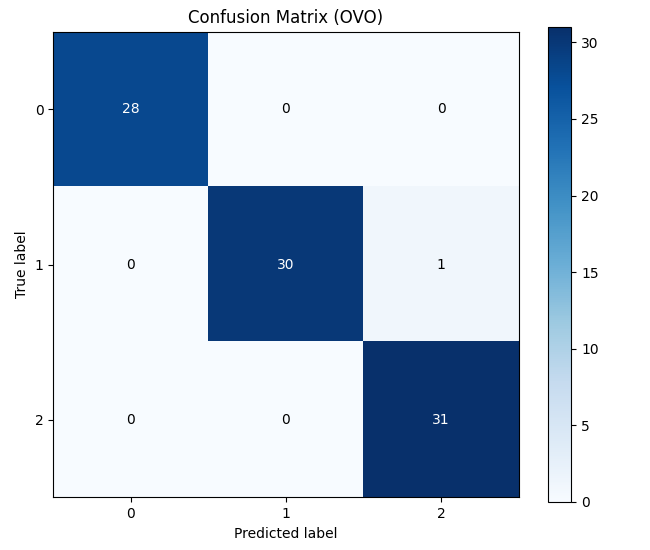
\includegraphics[scale=0.5]{output3.png}
		\caption{标准化后训练集与测试集的分布情况}
	\end{figure}
	
	再看决策边界图，OvO 方法把平面分成了三个主要区域，每个区域对应一个类别。图中可以看到，大部分测试样本都落在了正确的区域里，只有边界附近个别点会出现混淆。这也比较符合直觉，因为这些点本来就更靠近类别交界处，判错一点其实很正常。但通过引入核函数，边界变得更加复杂和灵活，能够更好地适应非线性问题。
	
	\begin{figure}[H]
		\centering
		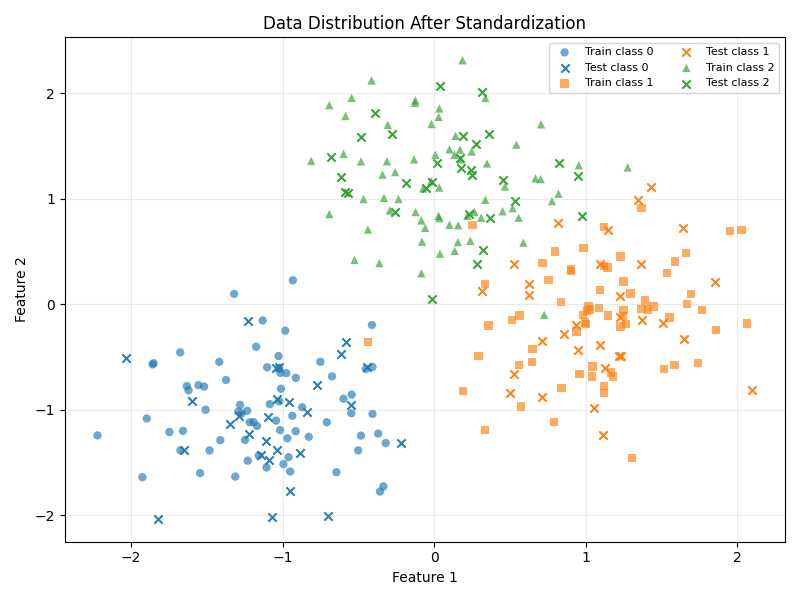
\includegraphics[scale=0.5]{output.png}
		\caption{OvO 策略下使用高斯核的决策边界}
	\end{figure}
	
	从混淆矩阵上进一步看，类别 0 和类别 2 基本都分对了，类别 1 有 1 个样本被分到了类别 2。这个结果说明模型已经能够把三类样本整体区分开，但边界附近还是会受到样本分布重叠的影响。不过与线性 SVM 不同的是，通过使用核函数，我们可以在更复杂的特征空间中进行分类，使得边界不再限于线性，从而能够更好地处理非线性问题。
	
	\begin{figure}[H]
		\centering
		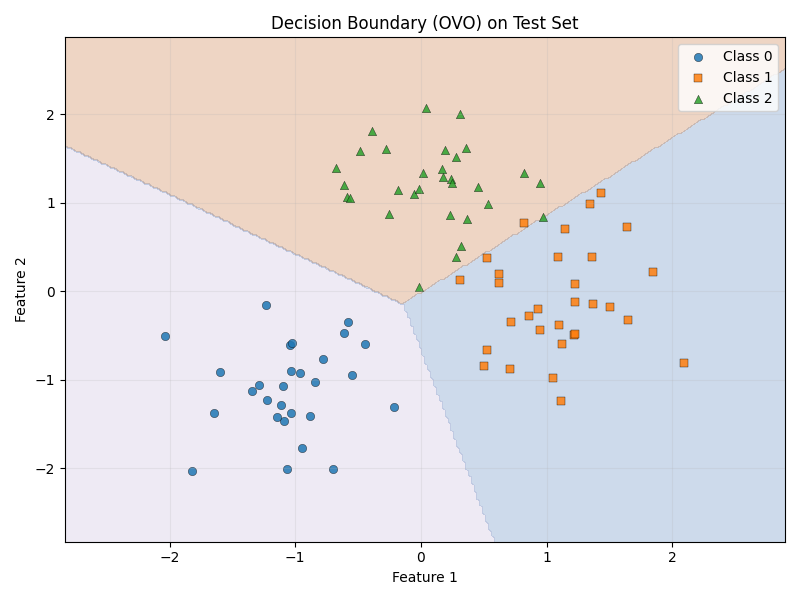
\includegraphics[width=0.72\textwidth]{output2.png}
		\caption{OvO 策略下使用高斯核的混淆矩阵}
	\end{figure}
	
	整体来看，这次实验的结果还是比较符合预期的。一方面，自己从零实现支持向量机并引入核函数后，对 Hinge loss、间隔最大化、核技巧、多分类投票这些概念会更有感觉；另一方面，通过参数搜索优化和可视化图像，能够直观地看到不同核函数对决策边界的影响，比较深入地理解了为什么高斯核在处理非线性问题时能够更好地适应数据。
	
	\section*{九、实验中遇到的问题与处理}
	这次实验相比之前涉及了更多的核函数、参数优化等问题：
	\begin{enumerate}
		\item 标签格式问题。 二分类 SVM 更新时更适合用 $\{-1,+1\}$ 作为标签，而原始多分类标签是 $\{0,1,2\}$。我在训练每个二分类器时，单独把当前任务对应的标签映射成了 $+1$ 和 $-1$。
		\item 多分类预测的整合问题。 OvR 和 OvO 的合并逻辑是不一样的：OvR 是比较分数选择最大的，OvO 是统计投票数选择多数。
		\item 核函数计算的效率问题。 对于高斯核等复杂核函数，计算两两之间的核值需要大量计算。本实验通过使用 NumPy 的向量化操作来加速计算。在决策函数计算时，使用 $f(x) = \sum\limits_{i=1}^m \alpha_i y_i \kappa(x, x_i) + b$ 形式，避免显式特征映射。
		\item 参数 $\gamma$ 的选择问题。 高斯核的带宽参数 $\gamma$ 对模型性能影响很大。太小的 $\gamma$ 会导致模型欠拟合，太大的 $\gamma$ 会导致过拟合。通过网格搜索可以找到合适的 $\gamma$ 值。
		\item 可视化问题。 对于高维特征，不能直接可视化。解决方法是在实验中使用低维数据集（如鸢尾花数据集）或使用 PCA 降维。
	\end{enumerate}
	
	\section*{十、实验总结}
	这次实验通过实现支持向量机算法，加强我们对核方法求解问题的理解。特别是核函数的引入，具有如下的意义：
	\begin{enumerate}
		\item 核函数的作用：通过定义合适的核函数，我们可以在隐含的高维特征空间中进行线性分类，而不需要显式计算高维特征，这大大降低了计算复杂度。
		\item 参数优化的重要性：不同的核函数和参数组合会显著影响模型的性能。通过网格搜索等系统的优化方法，我们能够找到最优的参数组合。
		\item 多分类策略的选择：OvR 和 OvO 各有优缺点，在实际应用中需要根据具体问题选择合适的策略。特别是在类别不平衡的场景下，OvO 往往表现更好。
	\end{enumerate}
\end{document}
